\documentclass[a4paper, 12pt]{article} % тип документа

%%%Библиотеки
	%\usepackage[warn]{mathtext}	
	\usepackage[T2A]{fontenc}   %Кодировка
	\usepackage[utf8]{inputenc} %Кодировка исходного текста
	\usepackage[english, russian]{babel} %Локализация и переносы
	\usepackage{caption}
	\usepackage{listings}
	\usepackage{amsmath, amsfonts, amssymb, amsthm, mathtools}
	\usepackage[warn]{mathtext}
	\usepackage[mathscr]{eucal}
	\usepackage{wasysym}
	\usepackage{graphicx} %Вставка картинок правильная
	\DeclareGraphicsExtensions{.pdf,.png,.jpg}
	\graphicspath{ {images/} }
	
	\setlength{\parskip}{0.5cm}
	
	\usepackage{pgfplots}
	\usepackage{indentfirst}
	\usepackage{float}    %Плавающие картинки
	\usepackage{wrapfig}  %Обтекание фигур (таблиц, картинок и прочего)
	\usepackage{fancyhdr} %Загрузим пакет
	\usepackage{lscape}
	\usepackage{xcolor}
	\usepackage[normalem]{ulem}
	\usepackage{wasysym}
	\usepackage{subfig}
	\usepackage{graphicx}
	
	\usepackage{titlesec}
	\titlelabel{\thetitle.\quad}

	\usepackage{hyperref}
	\newenvironment{comment}{}{}

%%%Конец библиотек

%%%Настройка ссылок
%%%	\hypersetup
%%%	{
%%%		colorlinks = true,
%%%		linkcolor  = blue,
%%%		filecolor  = magenta,
%%%		urlcolor   = blue
%%%	}
%%%Конец настройки ссылок


%%%Настройка колонтитулы
    \pagestyle{fancy}
    \fancyhead{}
    \fancyhead[L]{1.1.1}
    \fancyhead[R]{Засимов Георгий, группа Б01-109}
    \fancyfoot[C]{\thepage}
%%%конец настройки колонтитулы



\begin{document}

%%%Начало титульника
\begin{titlepage}

    \newpage
    \begin{center}
        \normalsize Московский физико-технический институт \\(национальный исследовательский университет)
    \end{center}

    \vspace{6em}

    \begin{center}
        \Large Лабораторная работа по общему курсу физики\\
    \end{center}

    \vspace{1em}

    \begin{center}
        \Large \textbf{Отчёт о выполнении лабораторной работы 1.2.5\\ {Изучение вынужденной регулярной прецессии гироскопа.}}
    \end{center}

    \vspace{2em}

    \begin{center}
        \large Засимов Георгий Алексеевич \\
        Группа Б01-109
    \end{center}

    \vspace{\fill}

    \begin{center}
    Долгопрудный \\2021
    \end{center}
    
\end{titlepage}
%%%Конец Титульника

\newpage




%\\\\\\\\\\\\\\\\\\\\\\\\\\\\\\\\\\\\\\\\\\\\\\\\\\\\\\\\\\\\\\\\\\\\\\\\\\\\
\section{Аннотация}

    В данной работе исследуется вынужденная прецессия гироскопа, устанавливается зависимость скорости вынужденной прецессии от величины момента сил, действующих на ось гироскопа, найденная скорость вращения ротора гироскопа сравнивается со скоростью, рассчитанной по скорости прецессии.






%----------------------------------------------------
\section{Теоретические сведения и методика измерений}



    Уравнение движения твёрдого тела можно записать в следующем виде:

\begin{equation}
\frac{d\vec{P}}{dt}=\vec{F}
\label{one}
\end{equation}

\begin{equation}
\frac{d\vec{L}}{dt}=\vec{M}
\label{two}
\end{equation}

    Момент импульса тела в главных его осях $x$, $y$, $z$ равен

\begin{equation}
\vec{L} = \vec{i}I_x\omega_x+\vec{j}I_y\omega_y+\vec{k}I_z\omega_z,
\label{three}
\end{equation}
    где $ I_x $, $ I_y $, $ I_z $ -- главные моменты инерции, $ \omega_x $, $ \omega_y $, $ \omega_z $ -- компоненты вектора угловой скорости $ \vec{\omega} $. Быстро вращающееся тело, для которого, например,

\[
I_z\omega_z \gg I_x\omega_x,\;\;\;\;I_y\omega_y,
\]

    принято называть гироскопом. Гироскоп называется уравновешенным, если его центр масс неподвижен.

    В силу \eqref{two} приращение момента импульса определяется интегралом

\begin{equation}
\Delta\vec{L} = \int\vec{M} dt.
\label{four}
\end{equation}

    Если момент внешних сил действует в течение короткого промежутка времени, из уравнения \eqref{four} следует, что приращение $ \Delta \vec{L} $ момента импульса значительно меньше самого момента импульса:

\[
\left|\Delta \vec{L}\right| \ll \left|\vec{L}\right| 
\]

\begin{center}
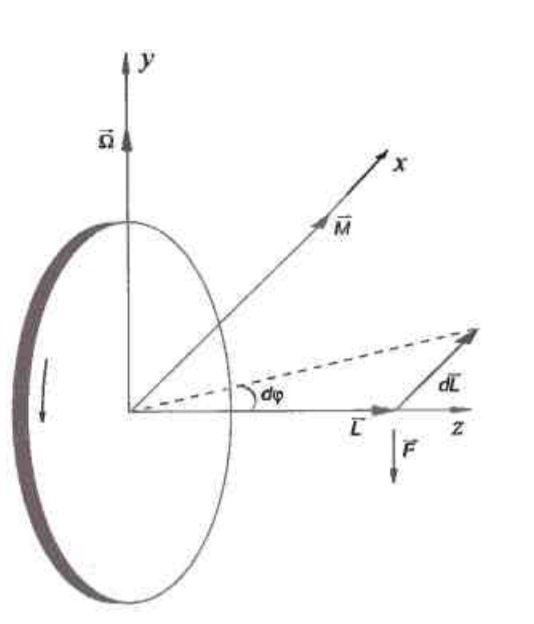
\includegraphics[width=4cm, height=5cm]{mahovik.jpeg}
\end{center}
\begin{flushright}
{\scriptsize \textbf{Рис. 1.} \textbf {Маховик.}}
\end{flushright}

    С этим связана замечательная устойчивость, которую приобретает движения
    гироскопа после приведения его в быстрое вращение. 
    Выясним, какие силы надо приложить к гироскопу, чтобы изменить
    направление его оси. Рассмотрим для 
    примера маховик, вращающийся вокруг оси $ z $, перпендикулярно
    плоскости маховика (рис. 1). Будем считать, что

\[
\omega_z = \omega_0, \;\;\;\;\; \omega_x = 0, \;\;\;\;\; \omega_y = 0.
\]

    \noindent Пусть ось вращения повернулась в плоскости $ zx $ по направлению к оси $ x $ на бесконечно малый угол $ d\varphi $. Такой поворот означает добавочное вращение маховика вокруг оси $ y $, так что

\[
d\varphi=\Omega dt,
\]

    где $ \Omega $ -- угловая скорость такого вращения. Будем предполагать, что

\begin{equation}
L_\Omega \ll L_{\omega_0}
\label{five}
\end{equation}

    Это означает, что момент импульса маховика, равный $ I_z\omega_0 $ до приложения внешних сил, только повернётся в плоскости $ zx $ по направлению к оси $ x $, не изменяя своей величины. Таким образом, 

\[
\left|d\vec{L}\right| = Ld\varphi = L\Omega dt.
\]

    Но это изменение направлено вдоль оси $ x $, поэтому вектор $ d\vec{L} $ можно представить в виде векторного произведения вектора угловой скорости $ \omega $, направленного вдоль оси $ y $, на вектор собственного момента импульса маховика, направленного вдоль оси $ z $,

\[
d\vec{L}=\vec{\Omega} \times \vec{L} dt,
\]

    т. е.

\[
\frac{d\vec{L}}{dt} = \vec{\Omega} \times \vec{L}.
\]

    В силу \eqref{two} имеем

\begin{equation}
\vec{M} = \vec{\Omega} \times \vec{L}.
\label{six}
\end{equation}

    Формула \eqref{six} справедлива, если выполнено условие \eqref{five}. Она позволяет определить момент сил $ \vec{M} $, который необходимо приложить к маховику для того, чтобы вызвать вращение оси маховика с угловой скоростью $ \vec{\Omega} $. Мы видим, таким образом, что для поворота оси вращающегося маховика к оси $ x $ необходимо приложить силы, направленные не вдоль оси $ x $, а вдоль оси $ y $, так чтобы их момент $ \vec{M} $ был направлен вдоль оси $ x $.

    Для гироскопа массой $ m_\text{г} $, у которого ось собственного вращения наклонена на угол $ \alpha $ от вертикали, скорость прецессии, происходящей вокруг вертикальной оси под действием силы тяжести, равна

\[
\Omega = \frac{M}{I_z\omega_0\sin \alpha} = \frac{m_\text{г}gl_\text{ц}\sin\alpha}{I_z\omega_0\sin\alpha} = \frac{m_\text{г}gl_\text{ц}}{I_z\omega_0},
\]

    где $ l_\text{ц} $ -- растояние от точки подвеса до центра масс гироскопа, т. е. скорость прецессии не зависит от угла $ \alpha $.

    Для изучения регулярной прецессии уравновешенного гироскопа к его оси подвешивают дополнительные грузы. Это смещает общий центр масс и создает момент сил тяжести, вызывающий прецессию. Скорость прецессии в этом случае равна

\begin{equation}
\Omega = \frac{mgl}{I_z\omega_0},
\label{eight}
\end{equation}

    где $ m $ -- масса груза, $ l $ -- расстояние от центра карданова подвеса до точки крепления груза на оси гироскопа.

    Измерение скорости прецессии гироскопа позволяет вычислить угловую скорость вращения его ротора. Расчет производится по формуле \eqref{eight}. Момент инерции ротора относительно оси симметрии $ I_0 $ измеряется по крутильным колебаниям точной копии ротора, подвешиваемой вдоль оси симметрии на жесткой проволоке. Период крутильных колебаний $ T_0 $ зависит от момента инерции $ I_0 $ и модуля кручения проволоки $ f $:

\[
T_0 = 2\pi\sqrt{\frac{I_0}{f}}.
\label{nine}
\]

    Чтобы исключить модуль кручения проволоки, вместо ротора гироскопа к той же проволоке подвешивают цилиндр правильной формы с известными размерами и массой, для которого легко можно вычислить момент инерции $ I_\text{ц} $. Для определения момента инерции ротора гироскопа имеем 

\begin{equation}
I_0=I_\text{ц}\frac{T_0^2}{T_\text{ц}^2},
\label{ten}
\end{equation}

    где $ T_\text{ц} $ --период крутильных колебаний цилиндра.\\
    
    
    
    
    
    
    
    
    
%---------------------------------------
\subsection{Экспериментальная установка}
    
    Для выполнения работы используется гироскоп (Рис. 2), закрепленный в карданном подвесе (Рис. 3).


\begin{center}
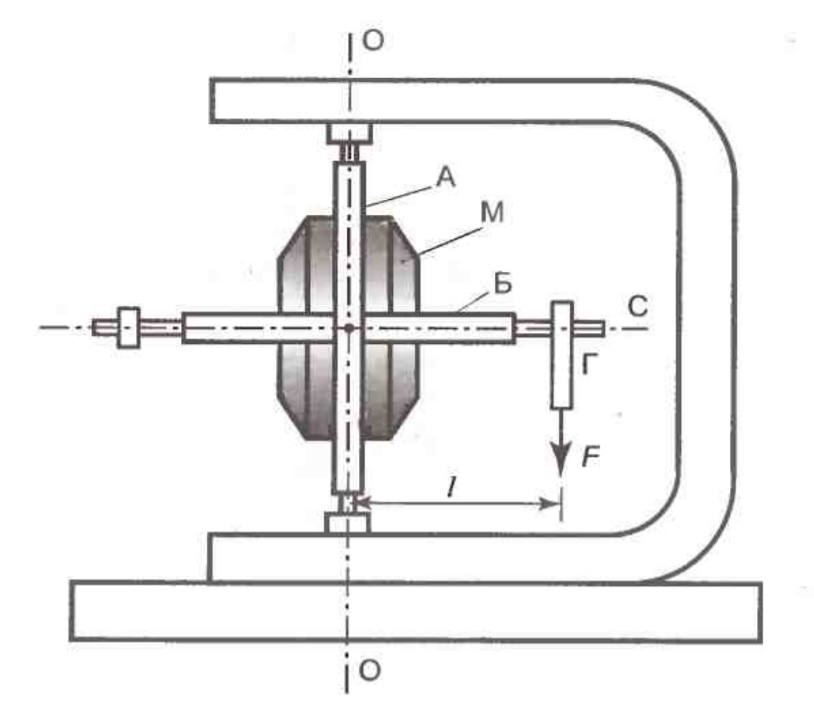
\includegraphics[scale = 0.18]{giroskop.jpeg}
\end{center}
\begin{flushright}
{\scriptsize \textbf{Рис. 2.} \textbf {Схема устройства гироскоп.}}
\end{flushright}

\begin{center}
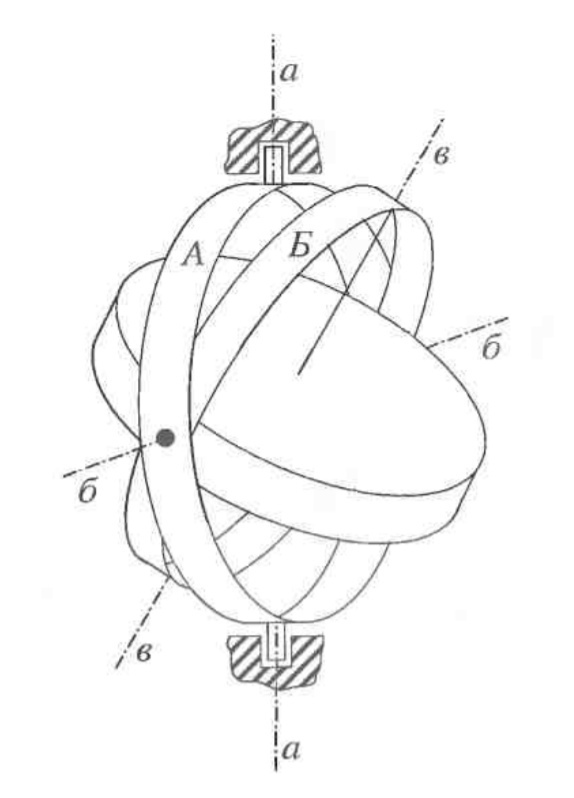
\includegraphics[scale = 0.18]{kard.jpeg}
\end{center}
\begin{flushright}
{\scriptsize \textbf{Рис. 3.} \textbf {Гироскоп, закрепленный в карданном подвесе..}}
\end{flushright}

    Ротором гироскопа (Рис. 2) является ротор электромотора М. Кожух мотора скреплен с кольцом Б (Рис. 3). Мотор с кольцом Б может вращаться в кольце А вокруг горизонтальной оси бб, которое может вращаться относительно оси аа. Рычаг С направлен по оси симметрии ротора. на рычаг подвешивают грузы Г.
    
    Направления моментов сил, инерции и угловых скоростей см на Рис.2.

%-----------------------------------------------------
\section{Оборудование и экспериментальные погрешности}


    \begin{itemize}
	\item Линейка: $ \sigma_\text{шт} = 0,001 $ м
	\item Секундомер: $ \sigma_\text{сек} = 0,5 $ с \textit{(с учётом реакции человека)}
	\item Электронные весы: $ \sigma_\text{вес} = 0,0001 $ кг
\end{itemize}




\section{Результаты измерений и обработка данных}

\subsection{Определение момента инерции ротора гироскопа}

    Для определения момента инерции цилиндра по формуле \eqref{ten} необходимо измерить период крутильных колебаний пробного цилиндра известной массы, вычислить его момент инерции и измерить период крутильных колебаний ротора гироскопа на той же проволоке.

\subsubsection{Вычисление момента инерции цилиндра}

    Момент инерции цилиндра вычисляем по формуле:

\[
I_\text{ц} = \frac{1}{2}m_\text{ц}\left( \frac{d_\text{ц}}{2}\right)^2,
\]

    где $ m_\text{ц} $ -- масса цилиндра, $ d_\text{ц} $ -- его диаметр.

    При измерении этих параметров получаем:
    
\begin{itemize}
	\item $ m_\text{ц} = \left( 1,617 \pm 0,0001\right) $ кг 
	$(\varepsilon_m = 0,01\%)$
	\item $ d_\text{ц} = \left( 0,081 \pm 0,001 \right) $ м
	$(\varepsilon_d = 1,2\%)$
\end{itemize}

    Тогда

\[
I_\text{ц} = 0,00133 \text{ кг} \cdot \text{м}^2
\]

    Погрешность вычисления момента инерции цилиндра может быть найдена по следующей формуле:

\[
\frac{\sigma_{I_\text{ц}}}{I_\text{ц}} = \sqrt{\left( \frac{\sigma_\text{m}}{m_\text{ц}} \right)^2 + \left(2 \frac{\sigma_\text{d}}{d_\text{ц}} \right)^2 } \approx 2,4 \%
\]

    В итоге получаем:

\begin{itemize}
	\item {$ I_\text{ц} = 0,00133 \pm 0,00003  \text{ кг} \cdot \text{м}^2 $, $ \left( \varepsilon =  2,4\% \right) $}
\end{itemize}






\subsubsection{Измерение периода крутильных колебаний пробного цилиндра}

    Производим измерение времени 15 крутильных колебаний цилиндра и повторяем опыт 6 раз. Полученные результаты заносим в таблицу 1.


\begin{table}[H]
\centering
\begin{tabular}{|l|l|l|l|c|c|c|}
\hline
№ & t, c  & N, раз & T, c  & \multicolumn{1}{l|}{\textless{}T\textgreater{}, c} & \multicolumn{1}{l|}{$\sigma_T$, c} & \multicolumn{1}{l|}{$\varepsilon_T$, \%} \\ \hline
1 & 61,25 & 15     & 4,083 & \multirow{6}{*}{4,059}                             & \multirow{6}{*}{0,0053}         & \multirow{6}{*}{0,13}                 \\ \cline{1-4}
2 & 60,69 & 15     & 4,046 &                                                    &                                 &                                       \\ \cline{1-4}
3 & 60,81 & 15     & 4,054 &                                                    &                                 &                                       \\ \cline{1-4}
4 & 60,78 & 15     & 4,052 &                                                    &                                 &                                       \\ \cline{1-4}
5 & 60,91 & 15     & 4,061 &                                                    &                                 &                                       \\ \cline{1-4}
6 & 60,84 & 15     & 4,056 &                                                    &                                 &                                       \\ \hline
\end{tabular}
\caption{Результат измерения периода крутильных колебаний цилиндра}
\end{table}

\label{formuli}


    Случайную погрешность определения периода крутильных колебаний рассчитываем по формуле:

\[
\sigma^{\text{сл}}_T = \sqrt{\frac{1}{N_\text{оп} - 1} \sum_{i = 1}^{N_\text{оп}} \left(T_i - \langle T \rangle \right)^2}.
\]

    Полная погрешность может быть вычислена по формуле:

\[
\sigma_T = \sqrt{\left( \sigma^\text{сл}_T \right)^2 + \left( \sigma_\text{сек} \right)^2  }
\]

    Получаем:

\begin{itemize}
	\item $ T_\text{ц} = \left( 4,059 \pm 0,005\right) $ с, $ \left(\varepsilon = 0,13 \% \right)  $
\end{itemize}





\subsubsection{Измерение периода крутильных колебаний ротора гироскопа}

    Производим измерение времени $ N_\text{кол} $ крутильных колебаний цилиндра и повторяем опыт 6 раз. Полученные результаты заносим в таблицу 2.


\begin{table}[H]
\centering
\begin{tabular}{|l|l|l|l|l|l|l|}
\hline
№ & t, c  & N, раз & T, c  & \textless{}T\textgreater{}, c & $\sigma_T$, c              & $\varepsilon_T$, \%      \\ \hline
1 & 63,69 & 20     & 3,185 & \multirow{6}{*}{3,213}        & \multirow{6}{*}{0,014} & \multirow{6}{*}{0,44} \\ \cline{1-4}
2 & 65,62 & 20     & 3,281 &                               &                         &                       \\ \cline{1-4}
3 & 64,16 & 20     & 3,208 &                               &                         &                       \\ \cline{1-4}
4 & 63,78 & 20     & 3,189 &                               &                         &                       \\ \cline{1-4}
5 & 64,12 & 20     & 3,206 &                               &                         &                       \\ \cline{1-4}
6 & 64,16 & 20     & 3,208 &                               &                         &                       \\ \hline
	\end{tabular}
	\caption{Результат измерения периода крутильных колебаний ротора гироскопа}
	\label{krut_gir}
\end{table}


    Получаем:

\begin{itemize}
	\item 
	$ T_0 = \left( 3,213 \pm 0,014 \right) $ с, $ \left( \varepsilon = 0,4 \% \right)  $
\end{itemize}





\subsubsection{Вычисление момента инерции ротора гироскопа}

По формуле \eqref{ten} вычислим момент инерции ротора гироскопа:

\[
I_0=I_\text{ц}\frac{T_0^2}{T_\text{ц}^2} = 0,00083 \text{ кг} \cdot \text{м}^2.
\]
Погрешность вычисления момента инерции ротора гироскопа:

\[
\frac{\sigma_{I_0}}{I_0} = \sqrt{\left( \varepsilon_{I_\text{ц}} \right)^2 +\left( 2 \varepsilon_{T_0} \right)^2 + \left(2 \varepsilon_{T_\text{ц}} \right)^2} \approx  2,5\%.
\]

В итоге получаем: \label{inertion}

\begin{itemize}
	\item $ I_0 = \left( 0,00083 \pm 0,00002 \right) \text{ кг} \cdot \text{м}^2, \left( \varepsilon = 2,5 \% \right) $
\end{itemize}






\subsection{Определение частоты вращения ротора гироскопа}

    Для определения частоты вращения ротора гироскопа будем исследовать зависимость скорости прецессии гироскопа от момента силы, действующей на его ось. Результаты измерений представлены в таблице 3.


\begin{table}[H]
\centering
\begin{tabular}{|l|l|l|l|l|l|l|l|l|l|}
\hline
№                  & m, г                 & М, Нм                      & t, c   & N, об & T, c    & \textless{}T\textgreater{}, c & $\varepsilon_T$          & $\Omega$, c^-1 & $\sigma_{Omega}$, c^-1 \\ \hline
\multirow{2}{*}{1} & \multirow{2}{*}{93}  & \multirow{2}{*}{0,1094796} & 169    & 1,5   & 112,667 & \multirow{2}{*}{111,131}      & \multirow{2}{*}{0,45} & \multirow{2}{*}{0,05651}     & \multirow{2}{*}{0,025}            \\ \cline{4-6}
                   &                      &                            & 219,19 & 2     & 109,595 &                               &                       &                              &                                   \\ \hline\hline
\multirow{2}{*}{2} & \multirow{2}{*}{116} & \multirow{2}{*}{0,1365552} & 130    & 1,5   & 86,667  & \multirow{2}{*}{87,899}       & \multirow{2}{*}{0,57} & \multirow{2}{*}{0,07145}     & \multirow{2}{*}{0,041}            \\ \cline{4-6}
                   &                      &                            & 222,83 & 2,5   & 89,132  &                               &                       &                              &                                   \\ \hline\hline
\multirow{2}{*}{3} & \multirow{2}{*}{142} & \multirow{2}{*}{0,1671624} & 105    & 1,5   & 70,000  & \multirow{2}{*}{70,767}       & \multirow{2}{*}{0,71} & \multirow{2}{*}{0,08874}     & \multirow{2}{*}{0,063}            \\ \cline{4-6}
                   &                      &                            & 214,6  & 3     & 71,533  &                               &                       &                              &                                   \\ \hline\hline
\multirow{2}{*}{4} & \multirow{2}{*}{173} & \multirow{2}{*}{0,2036556} & 88     & 1,5   & 58,667  & \multirow{2}{*}{58,702}       & \multirow{2}{*}{0,85} & \multirow{2}{*}{0,10698}     & \multirow{2}{*}{0,091}            \\ \cline{4-6}
                   &                      &                            & 234,95 & 4     & 58,738  &                               &                       &                              &                                   \\ \hline\hline
\multirow{2}{*}{5} & \multirow{2}{*}{214} & \multirow{2}{*}{0,2519208} & 78     & 1,5   & 52,000  & \multirow{2}{*}{49,824}       & \multirow{2}{*}{1,00} & \multirow{2}{*}{0,12604}     & \multirow{2}{*}{0,126}            \\ \cline{4-6}
                   &                      &                            & 190,59 & 4     & 47,648  &                               &                       &                              &                                   \\ \hline\hline
\multirow{2}{*}{6} & \multirow{2}{*}{270} & \multirow{2}{*}{0,317844}  & 57     & 1,5   & 38,000  & \multirow{2}{*}{37,876}       & \multirow{2}{*}{1,32} & \multirow{2}{*}{0,16580}     & \multirow{2}{*}{0,219}            \\ \cline{4-6}
                   &                      &                            & 188,76 & 5     & 37,752  &                               &                       &                              &                                   \\ \hline
\end{tabular}
	\caption{Результат измерения зависимости скорости прецессии от момента сил}
	\label{sk_pre}
\end{table}

    Момент силы, действующей на ось ротора гироскопа можно вычислить по следующей формуле ($l = 120$ мм):

\[
M = mgl.
\]

    Тогда погрешность вычисления момента силы определяется следующим соотношением:

\[
\sigma_M = M\sqrt{\left( \frac{\Delta_\text{вес}}{m} \right)^2 + \left( \frac{\Delta_\text{лин}}{l} \right)^2}
\]

    Период вращения гироскопа и погрешность его определения вычисляются по формулам, приведённым в п.п. \ref{formuli}.
    Тогда скорость прецессии гироскопа можно найти по формуле:

\[
\Omega = \frac{2\pi}{T}.
\]

    При этом погрешность вычисления скорости прецессии равна:
    
\[
\sigma_\Omega = \Omega \varepsilon_T.
\]

    Полученные результаты записываем в таблицу \ref{sk_pre}.

    Согласно уравнению \eqref{eight}, зависимость скорости прецессии $ \Omega $ от момента сил $ M $ должна быть линейной:

\[
\Omega = kM,
\]

    где
    
\[
k = \frac{1}{I_0\omega_0}.
\]

    Значит зависимость можно аппроксимировать с помощью метода наименьших квадратов. По полученным данным построим график зависимости. Он представлен на рисунке 4. Заметим, что точка, не принадлежащая прямой отклонена от предполагаемого значения в пределе 3$\sigma$. Данное несовпадение вызвано достаточно высокой погрешностью измерений и малым количеством боротов гироскопа в первой серии экспериментов.

\begin{figure}[H]
	\includegraphics[scale = 0.45]{omegaM.jpg}
	\caption{График зависимости скорости прецессии гироскопа от момента силы}
	\label{graph}
\end{figure}

    Коэффициент $ k $ можно вычислить по следующей формуле:\label{k}

\[
k = \frac{\langle M\Omega\rangle}{\langle M^2 \rangle}.
\]

    Случайную погрешность определения $ k $:

\[
\sigma^\text{сл}_k = \sqrt{\frac{1}{{(N_\text{оп}-1)}} \frac{\langle \Omega^2 \rangle}{\langle M^2 \rangle} - k^2} \approx 0,005 \text{ } \frac{1}{\text{Дж} \cdot \text{с}},
\]

    где $ N_\text{оп} = 6 $ -- число серий опытов.

    Систематическую погрешность определения $ k $ можно вычислить следующим образом:

\[
\sigma^\text{сист}_k = k\sqrt{\left( \frac{\sigma_M}{M} \right)^2+\left(\frac{\sigma_\Omega}{\Omega} \right)^2} \approx 0,0048 \text{ } \frac{1}{\text{Дж} \cdot \text{с}}.
\]

    Тогда полная погрешность определения $ k $ определяется следующим образом:

\[
\sigma_k = \sqrt{\left( \sigma_k^\text{сл} \right)^2 + \left( \sigma_k^\text{сист} \right)^2  } \approx 0,007 \text{ } \frac{1}{\text{Дж} \cdot \text{с}}.
\]

    Таким образом, получаем:

\begin{itemize}
	\item $ k =\left( 0,518 \pm 0,007 \right) \frac{1}{\text{Дж} \cdot \text{с}} , \left( \varepsilon = 1,35 \% \right) $
\end{itemize}

    С помощью $ k $ можно вычислить угловую скорость вращения ротора гироскопа:

\[
\omega_0 = \frac{1}{I_0 k} \approx 2325,9 \text{ с}^{-1},
\]
    
    где $ I_0 $ -- момент инерции ротора гироскопа, вычисленный в п.п. \ref{inertion}.

    Тогда погрешность вычисления $ \omega_0 $ можно определить по формуле:

\[
\frac{\sigma_{\omega_0}}{\omega_0} = \sqrt{\left( \frac{\sigma_{I_0}}{I_0} \right)^2 + \left( \frac{\sigma_k}{k} \right)^2} \approx 2,8 \%.
\]

    Таким образом, получаем:

\begin{itemize}
	\item {$ \omega_0 =\left( 2325,9 \pm 65,1 \right) \text{ с}^{-1} , \left( \varepsilon = 2,8 \% \right) $}
\end{itemize}

    Используя угловую скорость, можно определить частоту вращения ротора гироскопа:

\[
\nu = \frac{\omega_0}{2\pi} \approx 370,4 \text{ Гц}.
\]

    Погрешность определения частоты вращения вычисляется по следующей формуле:

\[
\sigma_\nu = \nu \varepsilon_{\omega_0} \approx 10,4 \text{ Гц}.
\]

    Таким образом, мы получили:

\begin{itemize}
	\item $ \nu = \left( 370,4 \pm 10,4 \right) \text{ Гц}, \left( \varepsilon = 2,8 \% \right)   $
\end{itemize}













\section{Определение частоты вращения ротора гироскопа при помощи осциллографа}

Скорость вращения ротора гироскопа можно определить и не прибегая к исследованию прецессии. У используемых в работе гироскопов статор имеет две обмотки, необходимые для быстрой раскрутки гироскопа. В данном случае одну обмотку используют для раскрутки гироскопа, а вторую -- для измерения числа оборотов ротора. Ротор электромотора всегда немного намагничен. Вращаясь, он наводит во второй обмотке переменную ЭДС индукции, частота которой равна частоте вращения ротора. Частоту этой ЭДС измеряем по фигурам Лиссажу, получаемым на экране осциллографа, если на один вход подать исследуемую ЭДС, а на другой — переменное напряжение с хорошо прокалиброванного генератора. При совпадении частот на экране получится неподвижный эллипс.\\
При настройке генератора сигнала на частоту \underline{$ \nu_0 = 400$ Гц} на экране осциллографа виден  практически неподвижный эллипс, следовательно эта частота сигнала совпадает с частотой вращения ротора гироскопа.


















\section{Оценка момента силы трения}

Для оценки момента силы трения, действующего на ось гироскопа, исследуем зависимость опускания оси гироскопа от времени. Результаты проведённых измерений записываем в таблицу 

\begin{table}[h!]
\centering
\begin{tabular}{|l|l|l|l|l|l|l|l|}
\hline
№ & $\alpha$, рад (14 C) & $\sigma_{\alpha}$, рад & t, c   & $\sigma t$, c & \textless{}T\textgreater{}, c & $\sigma_T$, c            & $\Omega$, rad/c           \\ \hline
1 & 0,244             & 0,017            & 169    & 0,5        & \multirow{2}{*}{194,095}      & \multirow{2}{*}{0,71} & \multirow{2}{*}{0,032} \\ \cline{1-5}
2 & 0,244             & 0,017            & 219,19 & 0,5        &                               &                       &                        \\ \hline
\end{tabular}
	\caption{Результат измерения зависимости опускания оси гироскопа от времени}
	\label{tab:my-table}
\end{table}

По полученным данным мы можем оценить момент силы трения, действующей на ось гироскопа по следующей формуле:

\[
M = \Omega I_0\omega_0 = \frac{\Omega}{k} \approx 10^{-3} \text{ } \text{Н} \cdot \text{м},
\]


    Тогда погрешность определения момента силы трения равна:

\[
\sigma_M = M\sqrt{\varepsilon_M^2+\varepsilon_\Omega^2} \approx 10^{-5} \text{ } \text{Н} \cdot \text{м}.
\]












\section{Выводы}

В ходе работы мы определили частоту вращения ротора гироскопа:$ \nu = \left( 370,4 \pm 10,4 \right) \text{ Гц}, \left( \varepsilon = 3,7 \% \right)   $
Полученная частота отличается от значения частоты, измеренного с помощью осциллографа ($ \nu_\text{осц} = 400 $ Гц) в пределах погрешности 3$\sigma$. Основной вклад в определение погрешности вносит погрешность определения угла отклонения горизонтальной оси гироскопа и погрешность определнеия момента инерции ротора.\\

Также был оценен момент силы трения, действующий на ось гироскопа $ M \approx 10^{-3} \text{ } \text{Н} \cdot \text{м} $. Он оказался достаточно мал по сравнению с моментом силы тяжести груза, подвешенного на ось гироскопа, но достаточным для поворота гироскопа в сторону направления силы тяжести груза. Для его более точной оценки необходима более точная шкала определения отклонения гироскопа от начального уровня.


















\end{document}
